\documentclass{article}
\usepackage{amssymb, amsmath, amsthm}
\usepackage[margin=1in]{geometry}
\usepackage{verbatim}
\usepackage{graphicx}
\usepackage{hyperref} % \url \href
\usepackage{docmute}

\newcommand{\pfrac}[2]{\frac{\partial #1}{\partial #2}}
\newcommand{\setM}{\mathcal{M}}
\newcommand{\bfx}{\mathbf{x}}
\newcommand{\bft}{\mathbf{t}}

\newtheorem*{theorem}{Theorem}
\newtheorem*{lemma}{Lemma}

\theoremstyle{remark}
\newtheorem*{remark}{remark}
\theoremstyle{remark}
\newtheorem*{example}{example}

\theoremstyle{definition}
\newtheorem*{definition}{Definition}

\DeclareMathOperator{\Aut}{Aut}
\DeclareMathOperator{\Image}{Im}
\DeclareMathOperator{\AO}{AO}
\DeclareMathOperator{\E}{E}
\DeclareMathOperator{\Sym}{Sym}
\DeclareMathOperator{\GL}{GL}
\DeclareMathOperator{\Hom}{Hom}
\DeclareMathOperator{\Tr}{trace}
\DeclareMathOperator{\Bij}{Bij}
\DeclareMathOperator{\Orb}{Orb}

% the highest level is part
% in each part, different section give different topics that are lossly connected
% subsection* should be used for giving subsequent definitions that are less important
\begin{document}

\title{Group Theory and Representation}
\author{Wenhao}
\date{\today}
\maketitle

\tableofcontents

\documentclass{amsart}
%\usepackage{amssymb, amsmath, amsthm}
\usepackage[margin=1in]{geometry}
\usepackage{verbatim}
\usepackage{graphicx}
\usepackage{hyperref} % \url \href
\usepackage{docmute}

\newcommand{\pfrac}[2]{\frac{\partial #1}{\partial #2}}
\newcommand{\setM}{\mathcal{M}}
\newcommand{\bfx}{\mathbf{x}}
\newcommand{\bft}{\mathbf{t}}

\newtheorem*{theorem}{Theorem}
\newtheorem*{lemma}{Lemma}

\theoremstyle{remark}
\newtheorem*{remark}{remark}
\theoremstyle{remark}
\newtheorem*{example}{example}

\theoremstyle{definition}
\newtheorem*{definition}{Definition}

\DeclareMathOperator{\Aut}{Aut}
\DeclareMathOperator{\Image}{Im}
\DeclareMathOperator{\AO}{AO}
\DeclareMathOperator{\E}{E}
\DeclareMathOperator{\Sym}{Sym}
\DeclareMathOperator{\GL}{GL}
\DeclareMathOperator{\Hom}{Hom}
\DeclareMathOperator{\Tr}{trace}
\DeclareMathOperator{\Bij}{Bij}
\DeclareMathOperator{\Orb}{Orb}

% the highest level is part
% in each part, different section give different topics that are lossly connected
% subsection* should be used for giving subsequent definitions that are less important
\begin{document}


\part{Group Theory}

\section*{Mapping}
In this note, mapping and function are used interchangably. 
% https://en.wikipedia.org/wiki/Bijection,_injection_and_surjection
\subsection*{Injective}
A mapping is called injective (one-to-one) if each element of the codomain is mapped by 
at most one element of the domain (arguments, input). 
For all $x,x' in X$, $f(x)=f(x')$ only if $x=x'$.

\subsection*{Surjective}
A function is surjective (onto), if each element of the codomain is mapped to by at least one element of 
the domain. That is, the image of of the domain equals the codomain. 
For all $y\in Y$, there exist an $x\in X$ so that $y=f(x)$.

\subsection*{Bijection}
If the function is both injective and bijective, than it is called bijective. Bijective is also called invertible.

\begin{figure}[h!]
    \centering
    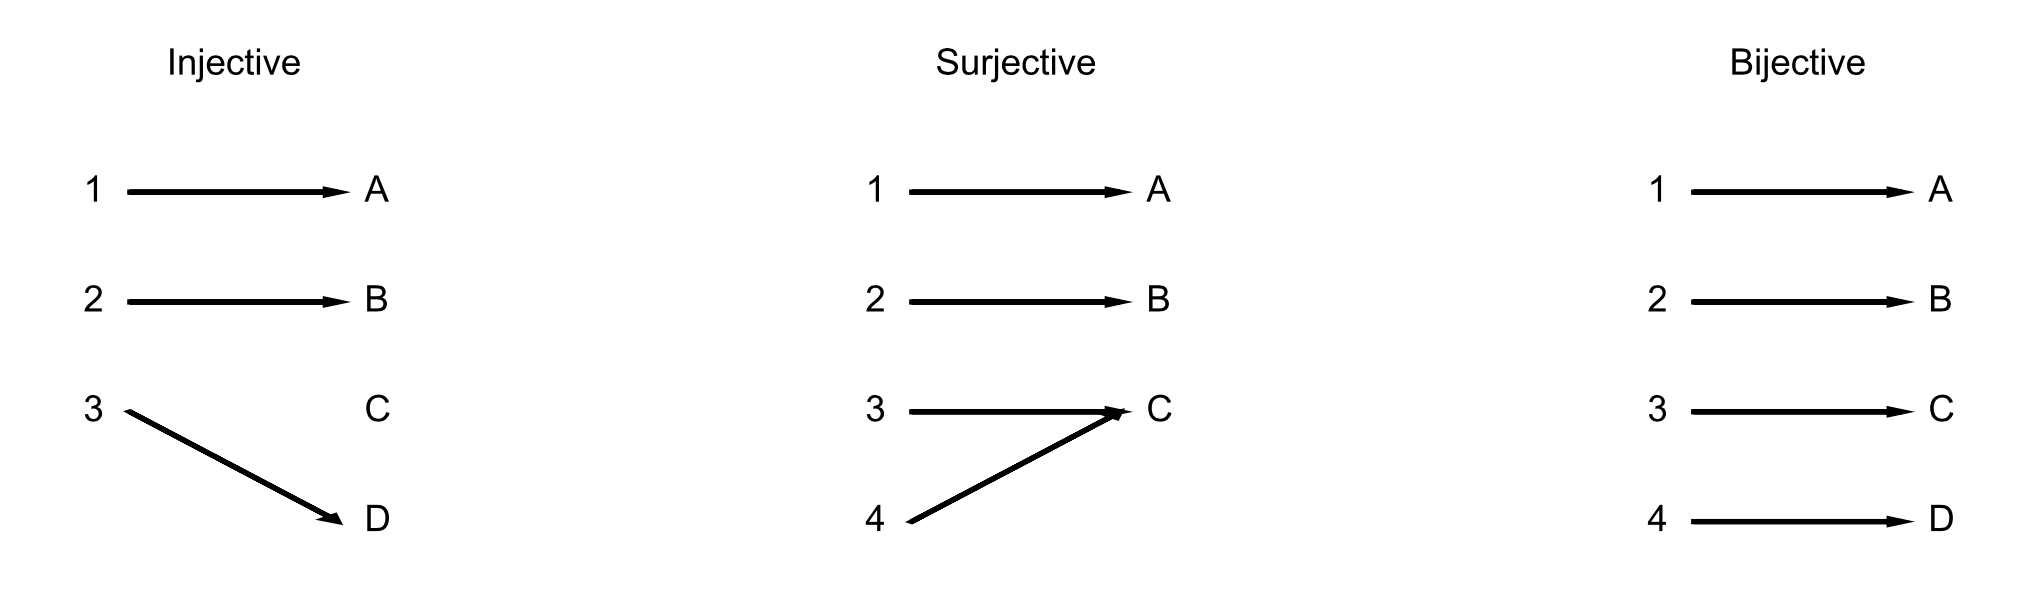
\includegraphics[width = 5in]{figures/mapping.png}
\end{figure}

\vspace{10pt}
\section*{Definition of Group}
\begin{definition}[Group]
    A group is a set plus an operation, that map an ordered pair of group element $(g,h)$ of $G$ into another element $g\cdot h \in G$, satisfying
    the following properties:
    \begin{enumerate}
        \item operation is associative: $g\cdot (h \cdot k) = (g\cdot h) \cdot k$ for $g,h,k \in G$;
        \item $G$ contain an identity element $e$, that satisfies $g\cdot e = e\cdot g = g$ for all $g \in G$ and 
        \item Each element of $G$ has an inverse, denoted by $g^{-1}$.
    \end{enumerate}  
\end{definition}

\subsection*{Order of the group}
    Order of the group $G$, or the cardinality of the group, is the number of elements in the set $G$, denoted by $|G|$


\vspace{10pt}
\section*{Two important group}

\subsection*{Linear transformation group}
Denoting $V$ as a vector space on field $F$, we write $\text{GL}(V)$ (general linear) as the set of all \emph{invertible linear transformation} in $V$. 
Since $g\in GL(V)$ is invertible and the product of two invertible linear transformation is again an invertible transformation, $GL(V)$ 
form a group. The group elements map a vector $v\in V$ to another vector $v' \in V$. Invertible means that the determinant of the 
matrices are non-zero.

\subsection*{Permutation group}
Denoting a set by $X$. All the bijections of $X$ to itself form a group, which we denote $\Sym(X)$. 

\vspace{10pt}

For a set $X$ with $n$ elements $|X| = n$, the total number of possible bijection (permutation) is $n!$. Therefore $|\Sym(X)| = n!$.
Since we care about bijections $X\to X$, not the set $X$ itself, Therefore, for two sets with the same number of elements,
$|X| = |Y|$, their permutation group is the same: $\Sym(X) = \Sym(Y)$ and we simply denote it as $\Sym(n)$ or $S_n$.

\subsubsection*{Two line notation of permutation}
We denote a permutation by $\pi\colon \{1,2,\dots,n\} \to \{ \cdots \}$. For example:
\[
    \pi = \left(  
    \begin{matrix} 
    1&2&3&4&5\\
    5&4&1&2&3
    \end{matrix}
    \right) \in S_5
\]
gives a permutation $\{1,2,3,4,5\} \to \{ 5,4,1,2,3 \}$. Such notation is called 'two-line notation'
We should note that the numbers are to be interpreted as indices of the objects in the set.

\subsubsection*{Matrix notation}
In matrix form, we have:
\begin{equation*}
    \left( \begin{matrix} 5 \\ 4 \\ 1 \\ 2\\ 3 \end{matrix} \right)
    = \left( \begin{matrix} 
        0 & 0 & 0 & 0 & 1 \\
        0 & 0 & 0 & 1 & 0 \\
        1 & 0 & 0 & 0 & 0 \\
        0 & 1 & 0 & 0 & 0 \\
        0 & 0 & 1 & 0 & 0 
    \end{matrix} \right) 
    \left( \begin{matrix} 1 \\ 2 \\ 3 \\ 4 \\ 5 \end{matrix} \right)
\end{equation*}
We call the matrix of permutation $A_{\pi}$. 
With the matrix notation, we can define the sign of a permutation:
\[\text{sign}\pi = \det A_{\pi}\]

\subsubsection*{Cyclic notation}
For the example permutation $\{1,2,3,4,5\} \to \{ 5,4,1,2,3 \}$, we can simply write
$\pi = (153)(24)$
The interpretion of cyclic notation is as follows:
\begin{itemize}
    \item a cyclic is a permutation of a subset without affecting other elements,
    \item fixed point can be omitted,
    \item $(153)$ is read as $1\to 5, 5\to 3, 3\to 1$. $1\to5$ reads 'object in position 1 become object in position 5'.
\end{itemize}
We can generate the two-line notation from the cyclic notation as follows:
\begin{equation*}
    \begin{matrix}
                & 1 & 2 & 3 & 4 & 5 \\
        1 \to 5 \quad & 5 &   &   &   &   \\
        5 \to 3 \quad &   &   &   &   & 3 \\
        3 \to 1 \quad &   &   & 1 &   &   \\
        2 \to 4 \quad &   & 4 &   &   &   \\
        4 \to 2 \quad &   &   &   & 2 &   \\
                & 5 & 4 & 1 & 2 & 3
    \end{matrix}
\end{equation*}

The following arrow form of permutation is also convenient to keep track of the operation, especially for successive 
application of permutations. Note that the arrow $5\to1$ reads 'the object in position 5 is moved to position 1'.
\begin{figure*}[!h]
    \centering
    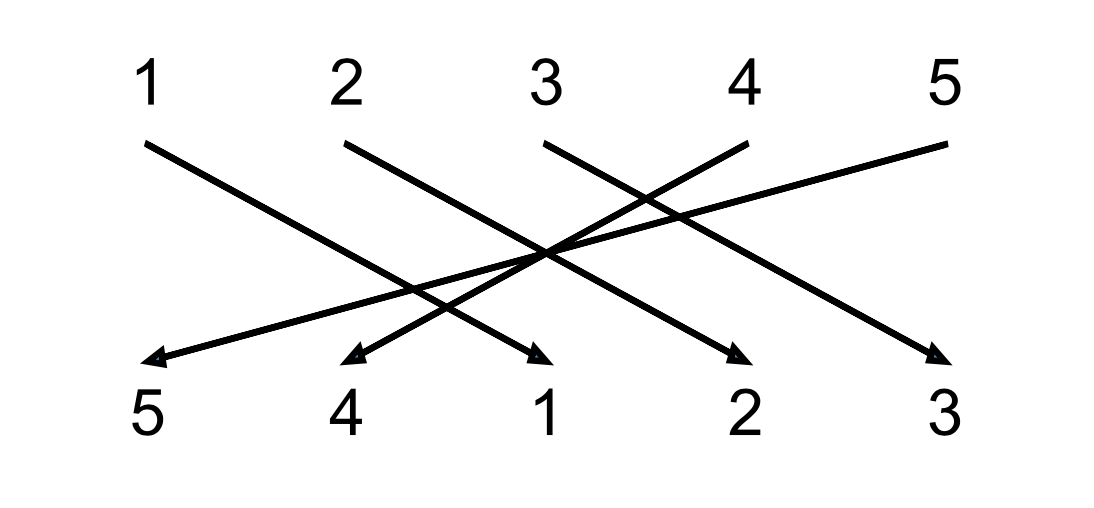
\includegraphics[width=2in]{figures/permutation_arrow.png}
\end{figure*}

\vspace{10pt}
\section*{Multiplication Table}
\subsection*{Multiplication Table}
Multiplication table shows how a group element are obtained by the product of two group element. We illustrate the multiplication 
table using the group $S_3$.
Using cyclic notation, we can write $S_3 = \{ e, (1,2), (2,3), (1,3), (1,2,3), (3,2,1) \}$. We have $|S_3| = 6$. The group table of $S_3$ can be calculated 
and tabulated to be:
\begin{table}[h]
    \centering
    \caption{Multiplication table of $S_3$}
    \begin{tabular}{|c|ccc|ccc|}
        \hline
                & e     & (123) & (321) & (12)  & (13)  & (23)  \\ \hline
           e    & e     & (123) & (321) & (12)  & (13)  & (23)  \\ 
          (123) & (123) & (321) & e     & (13)  & (23)  & (12)  \\
          (321) & (321) & e     & (123) & (23)  & (12)  & (13)  \\ \hline
          (12)  & (12)  & (23)  & (13)  &     e & (321) & (123) \\
          (13)  & (13)  & (12)  & (23)  & (123) & e     & (321) \\
          (23)  & (23)  & (13)  & (12)  & (321) & (123) & e     \\ \hline
    \end{tabular}
    \label{T:s3}
\end{table}

\begin{remark}
    We can varify for $S_3$, two elements $(12)$ and $(123)$ generate the whole group. 
    This result is also true for permutation group of higher order: For $S_n$, two elements
    $(12)$ and $(123\dots n)$ generate the whole group.
    (Not arbitrary two elements can generate the whole group: consider for $S_4$, two elements $(12)$ and $(23)$ will
    only permute index 1,2,3 but will not touch the fourth item. Of course, this two element generator set is not 
    the only generator set possible.)
\end{remark}

\vspace{10pt}
\section*{Subgroups}

\begin{definition}[Subgroup]
    Definition: $H$ is a non empty subset of $G$ and $H$ is a group, then $H$ is a subgroup of $G$
\end{definition}
For group $S_3$, we can find four non-trival subgroups: $\{e, (12)\}$, $\{e, (13)\}$, $\{e, (23)\}$ and $\{e, (123), (321)\}$

\begin{theorem}
    The intersections of subgroups of $G$ is also a subgroup of $G$.
\end{theorem}
\begin{proof}
    Suppose $H$ and $L$ are subgroups of $G$. $M$ is the intersections between $H$ and $L$, then:
    \begin{enumerate}
        \item identity $e \in M$;
        \item if $h_1, h_2 \in H$ and $h_1 \cdot h_2 = e$, If $h_1\in L$, then inevitably $h_2 \in L$, therefore the intersections of $H$ and $L$ is closed under inverse;
        \item similarly, if $h_1, h_2 \in H$ and $h_1, h_2 \in L$, then $h_1\cdot h_2$ belong to both $H$ and $L$ are therefore in the intersections. $M$ is closed under group operation.
    \end{enumerate}
\end{proof}

\begin{definition}[Generator]
    For a set $S$, the intersections of all subgroups contain $S$ is a subgroup. 
    This intersections is denoted by $\langle S\rangle$ and we say that it is generated by $S$. 
\end{definition}


For a group element $g$, we write that group that is generated by $g$ as $\langle g \rangle$, the order of $\langle g \rangle$ is also called the order of $g$. 

\subsection*{Cyclic group}
A group is called a cyclic group if it is generated by a single element, i.e., $G = \langle g \rangle$.

\begin{lemma}
    if a group $G$ is finite, we must have $g^n = e$ for $g \in G$. Since any $g^a$ is a number in $G$
\end{lemma}

\vspace{10pt}
\section*{Multiplication of group} 

\subsection*{Group multiplication}
For $S$ and $T$, both subset of group $G$, we define their product:
\begin{equation*}
    ST = \{st\mid s\in S, t \in T\}
\end{equation*}
and $sT \equiv \{s\}T $ and $Ts \equiv T\{s\} $ for $s \in S$.

\vspace{10pt}

\begin{definition}[Left cosets]
    For $H$ a subgroup of $G$ and $g \in G$, $gH$ is called a left coset. $Hg$ is called a right coset. 
    The set $\{gH \mid g \in G, H\ \text{is subgroup of}\ G\}$ is written as $G/H$
\end{definition}

For example, for $S_3$ and its subgroup $H = \{e,(123),(132)\}$, 
Using the multiplication table \ref{T:s3}, we can find that
applying element $g \in \{(12), (23), (13)\}$ on $H$
give the set $\{(12), (23), (13)\}$. Therefore, the left cosets of $H$ is:
\[
    \left\{\, \{e,(123),(132)\}, \{(12), (23), (13)\}\, \right\}    
\]

\begin{theorem}
    The left cosets of the subgroup $H$ of $G$ partition $G$
\end{theorem}
\begin{proof}
    This is equivalent to say that $gH$ is either $H$ itself, or share no comment elements with $H$.
    if $g\in H$, then $gH = H$. On the other hand, 
    if $g\notin H$ but $gh \in H$ for an element $h\in H$, then, by the requirement of group $h^{-1}\in H$. $ghh^{-1} = g \in H$ which conflict with the assumption.
    Therefore, we $gH$ cannot share element with $H$: $|gH| = |H|$, so that left cosets of a subgroup partition the group.
\end{proof}
As a result, the whole group can be written as:
\[
    G = H + g_1 H + g_2 H + \dots + g_n H    
\]
\begin{theorem}[Lagrange's theorem]
    For a finite group $G$ and $H$ is a subgroup of $G$, $|H|$ can divide $G$.
\end{theorem}
\subsection*{Index of $H$ in $G$}
    The number of left cosets of a subgroup $H$ is called the index of $H$ in $G$, denoted as $[G:H]$.
\begin{remark}
    If $G$ is a finite group and $g\in G$. Then the order of $\langle g\rangle$ divide $|G|$. This is because 
    $\langle g\rangle$ is a subgroup of G.
\end{remark}

\vspace{10pt}
\section*{Mapping}

\begin{definition}[Homomorphism]
    We define a mapping $\Phi\colon G \to H$ from group $G$ to $H$. If
    \[
        \Phi(g_1 g_2) = \Phi(g_1) \Phi(g_2)    
    \] 
    is satisfied for all $g_1, g_2 \in G$, then we call $\Phi$ a homomorphism
\end{definition}

\subsection*{Isomorphism}
    If the mapping $\Phi$ is a bijection, then we call $\Phi$ an isomorphism. If $G$ and $H$ are related by 
    an isomorphism, we write $G\cong H$

\begin{remark}
    Isomorphic groups have the same group multiplication table, apart from the names or symbols and, if necessary, after 
    rearranging rows and columns. 
    With the aid of isomorphism, all groups can be subdivided into \emph{isomorphism classes} of isomorphic groups. 
    Such a class is known as an \emph{abstract group}, each group within the isomorphism class are called 
    \emph{realization of the abstract group}
\end{remark}

\subsection*{Automorphism}
    We call the mapping $\Phi\colon G \to G$ (from $G$ onto itself) an automorphism. We write the set of all automorphism by $\Aut(G)$ 
\begin{remark}
Automorphism are bijections. For example, $\Phi\colon G \to gG$ is an automorphism, 
this is shown in the rearrangement theorem. 
\end{remark}

\vspace{10pt}

\begin{theorem}[Rearrangement theorem]
    for group $G$ and a group element $g'\in G$, the set 
    \[\{g'g \mid g \in G\}\]
    contain each group element once and only once.
\end{theorem}
\begin{proof}
    It is equivalent to say that if $g_1 \neq g_2$, then $g'g_1 \neq g'g_2$. all group element in $G$ are mapped 
    to another distinct elements in $G$ (rearrangement).

    If $g'g_1 = g'g_2$ but $g_1 \neq g_2$, then 
    \[ g'^{-1}g'g_1 = g'^{-1}g'g_2 \] which apperant conflict with the assumption
\end{proof}

\vspace{10pt}

\begin{definition}
    [Kernel] For a homomorphism $\Phi\colon G \to H$, we define the kernel $\ker\Phi = \{g\in G\mid \Phi(g) = e_h \}$, i.\,e.\,,
    kernel of $\Phi$ is the elements in $G$ that are mapped to identity of group $H$. $\ker\Phi \subset G$
\end{definition}

\begin{definition}
    [Image] For homomorphism $\Phi\colon G \to H$, we define the image $\Image\Phi = \{ \Phi(g) \mid g \in G \}$, i.\,e.\,,
    the elements in $H$ that are obtained from the mapping. $\Image\Phi \subset H$
\end{definition}

\begin{lemma}
    $\ker\Phi$ is a subgroup of $G$
\end{lemma}
\begin{lemma}
    $\Image\Phi$ is a subgroup of $H$
\end{lemma}

\vspace{10pt}

\begin{theorem}
    Homomorphism $\Phi\colon G\to H$ is injective if and only if $\ker \Phi = e$
\end{theorem}
\begin{proof}
    If $\Phi$ is injective, then we require $\ker \Phi = e_g$; 

    If $\ker \Phi = e_g$. Suppose $\Phi(a) = h$ and $\Phi(b) = h$. If in group $G$, we have $ax = b$, with $x\in G$, 
    Then we have:
    \[  
        \Phi(b) = \Phi(a)\Phi(x)    
    \]
    This implies that $\Phi(x)=e_h$ and $x = e_g$. Therefore, $a = b$: if $\ker \Phi = e_g$ then we cannot have
    two different elements in $G$ that are mapped to the same element in $H$.
\end{proof}

\vspace{10pt}
\section*{Conjugation of group elements}

\begin{definition}
    [Conjugate classes]
    Two group elements $a$ and $b\in G$ are called conjugate if there is another element $g$, so that:
    \[g^{-1}ag = b\]
    The elements of $g$ can then be collected into classes. $C_k$, each is made of conjugate elements. 
\end{definition}
\begin{remark}
    if $a$ is conjugate to $b$ and $b$ is conjugate to $c$, then $a$ is conjugate to $c$:
    \[ c = h^{-1}bh = h^{-1}g^{-1}agh = (gh)^{-1}a gh \]
\end{remark}
Conjugate partition $G$ into \emph{equivalent classes}. $C_a = \{g^{-1}ag\mid g\in G\}$ is called conjugacy class 
from $a$. 
As an example, for group $S_3$, with the help of multiplication table, we have the following conjugate classes:
\begin{align*}
    g^{-1}eg &= e  & (12)(123)(12) &= (321) & (12)(12)(12) = (12) \\
    &&  (13)(123)(13) &= (321) & (13)(12)(13) = (23) \\
    &&  (23)(123)(23) &= (123) & (23)(12)(123) = (13) \\
    &&  (321)(123)(123) &= (123) & (321)(12)(123) = (13) \\
    &&  (123)(123)(321) &= (123) & (123)(12)(321) = (23)
\end{align*}
Therefore, the conjugate classes are $\{e\}, \{(12),(23),(13)\}, \{(123),(321)\}$. 

We have the following general results for conjugate classes:
\begin{enumerate}
    \item Each element is at least conjugate to itself: $g^{-1}gg = g$,
    \item Every element in $G$ belongs to exactly one conjugacy class,
    \item Numbers of elements in conjugacy classes are different, but they are always divisor of order of $G$,
    \item Elements in the same conjugacy class have the same order.
\end{enumerate}

\subsection*{Self-conjugate elements}
If for $g_i\in G$ and we have $g_m^{-1}g_i g_m = g_i$ for all $g_m \in G$, then $g_i$ is called \emph{self-conjugate}.
\begin{remark}
    Since $g_m^{-1}g_i g_m = g_i$ means $g_i g_m = g_m g_i$, self-conjugate condition means that $g_i$ commute with all 
    elements in the $G$. 
    It is straightforward to see that identity element is always self-conjugate. 
\end{remark}

\subsection*{Abelian group}
A group is called abelian if for all $g, h \in G$, $g\cdot h = h \cdot g$. 
Therefore, each element $g\in G$ form a conjugate classes by its own.

\vspace{10pt}
\section*{Conjugating subgroups and Quotinet group}

Previous definition of conjugating is defined on elements. For subgroups, we also have similar definitions:
\begin{definition}
    [Conjugate subgroups]
    Two subgroup $H$ and $H'$ are called conjugate subgroups in $G$ if there exist an element $g_i\in G$
    so that $H' = g_i^{-1}Hg_i$, i.e., the left coset and the right coset formed from $H$ and $g_i$ are the same. 
\end{definition}
\begin{remark}
    The set of subgroups that are conjugate to $H$ form a conjugacy class. 
    The conjugate subgroups are isomorphic and have the same order.
\end{remark}
From the multiplication table of $S_3$, we find conjugating subgroups:
\begin{equation*}
    \overbrace{\{e, (123), (321)\}}\quad \overbrace{\{e, (12)\},\{e, (13)\},\{e, (23)\}}
\end{equation*}

\begin{definition}
    [Normal subgroup]
    A subgroup is called normal (self-conjugate) if 
    \[
        gHg^{-1} = H\quad \text{for all}\ g \in G 
    \]
    Equivalently, this means that every left cosets of $H$ in $G$ is also a right coset of $H$ in $G$.
\end{definition}
We can see that the subgroup $\{e, (123), (321)\}$ of $S_3$ is a normal subgroup: it only conjugate with itself.

If $H$ is a normal subgroup, then for the set $G/H$, we can show that $(g_1 H)\cdot(g_2 H)$ is also in 
set $G/H$:
\begin{proof}
    Since $H$ is a normal subgroup, by definition: 
    \[gH = Hg = gHg^{-1}g\] so that we fine:
    \[gHg^{-1} = H\]
    Then:
    \begin{align*}
        (g_1 H)\cdot(g_2 H) &= g_1 H g_1^{-1}g_1 g_2 H = H g_1 g_2 H \\
            &= (g_1g_2)(g_1g_2)^{-1} H (g_1g_2) H \\
            &= g_1g_2 H H = g_1 g_2 H 
    \end{align*}
    since $g_1 g_2 H$ is also a left coset and belong to $G/H$, we have shown that the set $G/H$ is indeed a group with 
    operation $(g_1 H)\cdot(g_2 H)$
\end{proof}

we call the group $G/H$ \textbf{quotinet group}, or factor group.
For example, for $H = \{e,(123),(132)\}$, the set ${H, (12)H}$ is the factor group.

\begin{lemma}
    The kernel $\ker\Phi$ of $\Phi\colon G\to H$ is a normal subgroup.
\end{lemma}

\begin{lemma}
    For a group homomorphism $\Phi\colon G\to H$, the quotinet group is isomorphic to $\Image\Phi$ (bijection).
\end{lemma}

\vspace{10pt}

\begin{definition}
    [Inner Conjugation]
    We call the mapping $\Phi_g\colon G\to G$ with $\Phi_g(h) = ghg^{-1}$ a conjugation with $g$, or an \emph{inner conjugation}
\end{definition}
According to definition, $\Phi_g \in \Aut(G)$


\vspace{10pt}
\section*{Action of a group}

\begin{definition}
    [Action of a group]
    For a group $G$ and a set $\setM$, the action of $G$ on $\setM$ is a mapping 
    $\alpha\colon G\times \setM \to \setM$ satisfying:
    \begin{enumerate}
        \item $\alpha(e,m) = m$ for $m \in \setM$;
        \item $\alpha(g, \alpha(h,m)) = \alpha(gh, m)$ for $m\in \setM$ and $h,g\in G$
    \end{enumerate}
\end{definition}
where $\alpha(g,m)$ means action of a group element $g$ on a set element in $\setM$

\begin{remark}
For an action of the group $\alpha$, 
we have a group homomorphism that map the the group actions to permutations on $\setM$. 
(Recall that permutations on $\setM$ is all the bijection that map $\setM$ to itself.) 
The homomorphism $\theta\colon G \to \Bij(\setM)$ is given by:
\begin{equation*}
    g\to (m\to \alpha(g,m))
\end{equation*}
$m\to \alpha(g,m)$ being a permutation.     
\end{remark}

\begin{definition}
    [Symmetry]
    A group element $g\in G$ is called a symmetry on set $\setM$ if it leave the set invariant:
    $\setM = \{gm \mid \text{for all }\ m \in \setM\}$. 
\end{definition}

\begin{comment}
\subsection*{Group action on itself}
For a group $G$, $G$ can act on itself by conjugation: $\alpha\colon G\times G \to G$ given by
$\alpha(h,g) = hgh^{-1}$

\begin{definition}
    [Symmetry]
    For a group $G$ acting on $\setM$, $T\subset M$ is called invariant under $S \subset G$ if $ST\subset T$, 
    with $ST = {\alpha(g,m)\mid g \in G, m\in T}$. 
    The elements in $S$ are called 'symmetry'.
\end{definition}

\end{comment}
\vspace{10pt}

\begin{definition}
    [Orbit under $G$]
    For $G$ acting on $\setM$, the sets $\Orb(m) = \{gm\mid g\in G\}$ partition the set $\setM$. 
    \[\setM = \Orb(m_1) + \Orb(m_2) + \dots + \Orb(m_n)\]
    Each set $\Orb(m)$ is called the orbit of $m$ under $G$.
\end{definition}

\subsection*{Transitive}
A group action, of $G$ on $\setM$, is called transitive if it has only one orbit, i.e., 
$\setM = \{gm \mid g \in G\}$ for some choice of $m$. A group is called transitive if 
its group action is transitive. 
The set $\setM$ of a transitive group action is called \emph{homogeneous space} if the group 
is a lie group.

\subsection*{Stabilizer}
For group $G$ acting on $\setM$ and $m \in \setM$, the set 
\[G_m = \{ g\in G\mid gm = m \}\]
are called the stabilizer of $m$. $G_m \subset G$
\footnote{stabilizer $G_m$ is not necessarily a normal subgroup of $G$}

\begin{lemma}
    Stabilizer $G_m$ is only normal if $G_m$ is also the stabilizer of every orbits of $m$: 
    if $g\in G_m$ stabilize any orbit of $m$ generated by $t\in G$, 
    we have: $gtm = tm$ and thus $t^{-1}gtm = m$. So that $t^{-1}gt \in G_m$ and $G_m$ is self-conjugating. 
    % https://proofwiki.org/wiki/Stabilizer_is_Normal_iff_Stabilizer_of_Each_Element_of_Orbit
\end{lemma}

\begin{theorem}
    [Orbit-Stabilizer theorem]
    The stabilizer $G_m$ is a subgroup of $G$, therefore, $|G_m|$ divide $G$. 
    Further more, $G_m$ is a normal subgroup. It's left cosets form a quotinet group $G/G_m$. 
    The mapping $f\colon \Orb(m) \to G/G_m$ is a bijection and $|G|=|G_m||\Orb(m)|$
\end{theorem}
\begin{remark}
    We call a
    subset of $\setM$ \emph{fundamental set} if it contain exactly one element from each orbit.
\end{remark}

\vspace{10pt}
\section*{Isometry}
The distance in euclidean space is given by 
\[
    d(x,y) = \|x-y\| = \sqrt{\sum_i(x_i-y_i)^2}    
\]

\begin{definition}
    [Isometry]
    A invertible mapping $g\colon \mathbb{E}^n \to \mathbb{E}^n$ satisfying 
    \begin{equation*}
        d(g(x),g(y)) = d(x,y)
    \end{equation*}    
    is called an isometry, i.e., the transformation that keep the distance. 
    We denote them $\E(n)$
\end{definition}
\begin{remark}
    See definition below, isometry is an affine transformation, can be written as AO(3).
    % http://math.soimeme.org/~arunram/Notes/afforth.html
\end{remark}

\begin{lemma}
All isometries of euclidean space that fix the origin are orthogonal linear map $O(N)$
\end{lemma}
A linear map is orthogonal if it perserves the inner product $x^T\cdot y$, therefore, linear 
orthogonal transformation satisfy:
\begin{equation*}
    (Mx)^T(My) = x^T M^{T}My = x^T y
\end{equation*}
therefore, an orthogonal transformation satisfy $M^{T}M = I$. 
We call $M$ \emph{orientation preserving} if it has determinant 1 (rotations) and 
\emph{orientation reversing} if it has determinant -1. The subgroup of O(N) with 
determinant 1 is denoted as special orthogonal group $SO(N)$

\begin{remark}
    We have a group homomorphism: $\epsilon\colon G \to \{-1, 1\}$ where the mapping is 
    given by the determinant. It is equivalent to the quotinet group $\{N, iN\}$ where 
    $N$ is the set of orientation preserving elements. $N$ is a normal subset of $G$ with 
    index 2, i.e., the number of elements in $N$ is half of in $G$. 
\end{remark}


\vspace{10pt}
All the translations $t_a\colon x \to x+a$ are also isometries of euclidean space. 
The following list gives all the possible isometries of $\mathbb{E}^3$: 
\begin{enumerate}
    \item Identity,
    \item a translation,
    \item a rotation around a rotation axis,
    \item a screw rotation,
    \item a reflection in some plane, 
    \item a glide reflection, and, 
    \item rotatory reflection (rotation followed by reflection in the plane perpendicular to rotation axis)
\end{enumerate}
\begin{remark}
Inversion is implicitly included in the list as a rotation refection of 180 degree:
\begin{equation*}
    i=C_2 \cdot m = \left(\begin{matrix}
        -1 & 0 & 0\\
        0  & -1 & 0\\
        0 & 0 & 1
    \end{matrix}\right) \cdot \left(\begin{matrix}
        1 & 0 & 0\\
        0  & 1 & 0\\
        0 & 0 & -1
    \end{matrix}\right)
\end{equation*}
\end{remark}

\vspace{10pt}

\begin{theorem}
    For an isometry $A$, there exist a vector $v$ and an orthogonal matrix $B$ so that 
    \begin{equation*}
        A(x) = B(x) + v 
    \end{equation*}
    i.e., any isometry is an orthogonal linear map followed by translation.
\end{theorem}

We can therefore define a group homomorphism: $\phi\colon E(N)\to O(N)$ given by $A\to B$. 
The group of translation is the kernel. Translation is also a normal subgroup.

\vspace{10pt}
\section*{Lattice}
\begin{definition}
    [Metric space]
    A set $\setM$ is a metric\footnote{metric means measureable} space if the distance (metrix function) 
    is defined to satisfying:
    \begin{enumerate}
        \item The distance between $a, b \in \setM$ $d(a,b)$ is positive if $a$ and $b$ is distinct, otherwise it is zero,
        \item The distance $d(a,b)$ is equal to that of $d(b,a)$, and 
        \item $d(a,b) \leq d(a,c) + d(c,b)$ with $c$ a third point.
    \end{enumerate}
\end{definition}

In point $x$ in a metric space is isolated if there is no other point in $\setM$ in its 
neighbourhood. $d(x,y)> \delta \quad \text{for all } y\in\setM \text{ except x itself}$.
A metric space is called \emph{discrete} if all its point is isolated. A group $G$ is called 
a discrete group if it act on discrete metric space. 

\begin{definition}
    [Lattice]
    We call a discrete additive subgroup of $\mathbb{R}^N$ a lattice in $\mathbb{R}^N$
\end{definition}
\begin{remark}
Lattice defined above is a subgroup of $\mathbb{R}^N$, 
i.e., lattice is a set of vectors in $\mathbb{R}^N$
\end{remark}

\begin{definition}
    [Crystallographic group]
    Crystallographic group $G$ is a subgroup of the group of all isometries, that has group 
    homomorphism:
    \begin{equation*}
        \phi\colon G \to O(N)
    \end{equation*}
    with kernel of discrete group of translations. The image of the homomorphism $\Image(\phi)$
    is called the \emph{Crystallographic point group}. 
    The discrete group of translation gives a lattice.
\end{definition}

\begin{comment}

\vspace{10pt} %%%%%%%%%%%%%%%%%%%%%%%%%%%%%%%%%%%%

For a subgroup $G\subset \AO(n)$, the map $R\colon G \to R(G)$ with $R(G)\in \text{O}(n)$ given by
$g = t_a R(g)$ is a group homomorphism. It's kernel is $T(G)$:
\begin{equation}
    T(G) = \{ a \in \mathbb{R}^n \mid t_a \in G\}
\end{equation}
the set of all translation. 

\begin{lemma}
    $T(G)$ is invariant under $R(G)$
\end{lemma}
i.\,e.\,, the application of $r\in R(G)$ on $t\in T(G)$ gives another translation in $T(G)$

\vspace{10pt} %%%%%%%%%%%%%%%%%%%%%%%%%%%%%%%%%%%%

\begin{definition}
    [Lattice]
    a discrete subgroup of $\mathbb{R}^n$ is called Lattice (with $+$ as group operation). The dimension of its span is called rank.
\end{definition}
Let $a_1,\dots,a_k \in \mathbb{R}^n$ be linearly independent, then the set 
$L = \sum_i \mathbb{Z} a_i$ is a lattice.

A subgroup $G\subset \AO(n)$ act discretely if all orbits in $\mathbb{R}^n$ is discrete.

\begin{lemma}
    If $G$ is a subgroup of $\AO(n)$ leaving a lattice $T$ invariant, then $G$ is finite
\end{lemma}

\begin{definition}
    [Crystallographic group]
    If $G$ is a subgroup of $\AO(n)$ for which $T(G)$ is the lattice translation, then $G$ is called 
    a crystallographic group.
\end{definition}
\subsection*{Crystallographic point group}
If $G\subset \text{O}(n)$ leave invariant a lattice of rank $n$, then $G$ is called a crystallographic point group

\begin{lemma}
    If $G$ is a crystallographic group, then $R(G)$ is a crystallographic point group
\end{lemma}
\end{comment}

\newpage


\end{document}

\documentclass{amsart}
%\usepackage{amssymb, amsmath, amsthm}
\usepackage[margin=1in]{geometry}
\usepackage{verbatim}
\usepackage{graphicx}
\usepackage{hyperref} % \url \href
\usepackage{docmute}

\newcommand{\pfrac}[2]{\frac{\partial #1}{\partial #2}}
\newcommand{\setM}{\mathcal{M}}
\newcommand{\bfx}{\mathbf{x}}
\newcommand{\bft}{\mathbf{t}}

\newtheorem*{theorem}{Theorem}
\newtheorem*{lemma}{Lemma}

\theoremstyle{remark}
\newtheorem*{remark}{remark}
\theoremstyle{remark}
\newtheorem*{example}{example}

\theoremstyle{definition}
\newtheorem*{definition}{Definition}

\DeclareMathOperator{\Aut}{Aut}
\DeclareMathOperator{\Image}{Im}
\DeclareMathOperator{\AO}{AO}
\DeclareMathOperator{\E}{E}
\DeclareMathOperator{\Sym}{Sym}
\DeclareMathOperator{\GL}{GL}
\DeclareMathOperator{\Hom}{Hom}
\DeclareMathOperator{\Tr}{trace}
\DeclareMathOperator{\Bij}{Bij}
\DeclareMathOperator{\Orb}{Orb}

% the highest level is part
% in each part, different section give different topics that are lossly connected
% subsection* should be used for giving subsequent definitions that are less important
\begin{document}

\part{Crystal Structure}
\section*{Lattice}
We consider a \emph{crystal structure} as the following object:
\begin{definition}
    [Crystal Pattern]
    The infinite, three-dimensional periodic array corresponding to a crystal is called \emph{crystal pattern}.
    The lengths of the periodicity may not be arbitrarily small. Crystal pattern is also known 
    as \emph{infinite ideal crystal}.
\end{definition}
We further distinguish two other concepts:
\begin{itemize}
    \item \emph{Macroscopic crystal} is a finite block of a crystal pattern,
    \item \emph{real crystal} has a finite size, but also defects.
\end{itemize}

\subsection*{Translation}
A shift which bring the crystal structure to superposition with itself is called 
a \emph{symmetry translation} or simply translation for this crystal structure. 
It is specified by a translation vector.

\begin{definition}
    [Vector lattice]
    The infinite set of all translation vectors $\bft_i$ of a crystal pattern is its \emph{vector lattice} $\mathbf{T}$, 
    or simply the \emph{lattice}. 
    The vectors are called \emph{lattice vectors}
\end{definition}
We distinguish vector lattice from the following two concepts:

\subsection*{Point lattice}
Choosing a starting point $\bfx_0$, the set of all the end points $\{\bfx_i\mid\bfx_i = \bfx_0 + \bft_i\}$
is call the \emph{point lattice} belongs to $\bfx_0$ and $\mathbf{T}$.
\subsection*{Particle lattice}
If the chosen point of a point lattice correspond to center of gravity of particles. Then we call this point lattice \emph{particle lattice}

The points that are related by translations are called \emph{translation equivalent}.

\vspace{10pt}
\section*{Basis and unit cell}

\subsection*{Basis}
To describe position in three-dimensional space, we need to choose an origin and a basis. 
A basis that consists of three lattice vectors of a crystal pattern is called a \emph{crystallograhic basis}
or a \emph{lattice basis} of the crystal structure. 

We further define the following terms:
\begin{itemize}
    \item \emph{Conventional basis} are the crystallograhic basis used in the International Tables A.
    \item \emph{Primitive basis} are the basis $a$, $b$ and $c$ with which every lattice vector $\bft$ can be expressed 
            as a linear combination with integral coefficients: $\bft = t_1 a + t_2 b + t_3 c$
\end{itemize}
A lattice is called \emph{primitive} if its conventional basis is primitive,  otherwise, we call it \emph{centred}. 

\subsection*{Unit cell}
A region in which all the points have coordinates \[0 \leq x,y,z < 1\]
with respect to its chosen basis and origin is called a \emph{unit cell} of the crystal structure.

\vspace{10pt}
\section*{Symmetry operations}

\begin{definition}
    [Symmetry operation]
    A symmetry operation is a mapping of an object such as 1) all distances remain unchanged and 2) the obejct is mapped onto itself or its mirror image.
    If the obejct is a crystal structure, the mapping is called a \emph{crystallographic symmetry operation}.
\end{definition}

\subsection*{Space group}
The set of all symmetry operations of a crystal structure is called the space group of the crystal structure.

\vspace{10pt}

\begin{definition}
    [Affine mapping]
    A mapping of space which maps parallel straight lines onto parallel straight lines is called an affine mapping. They do not necessary perserve 
    distance or angles.
\end{definition}

After choosing a coordination system, an affine mapping can always be represented as:
\begin{equation*}
    \left( \begin{matrix}
        a'\\b'\\c'
    \end{matrix} \right)  = \left( \begin{matrix}
        w_{11} & w_{12} & w_{13} \\
        w_{21} & w_{22} & w_{23} \\
        w_{31} & w_{32} & w_{33}
    \end{matrix} \right) \left( \begin{matrix}
        a\\b\\c
    \end{matrix} \right)+ \left( \begin{matrix}
        w_1\\w_2\\w_3
    \end{matrix} \right)
\end{equation*}
or simply, in matrix notation $\bfx' = W\bfx + w$. Affine mapping are Linear transformations.

\subsection*{Fixed point} A point $\bfx_F$ that is mapped onto itself is called a fixed point of the mapping.

\vspace{10pt}

\begin{definition}
    [Isometry]
    An affine mapping that leaves all distances and angles unchanged is called \emph{isometry}
\end{definition}
For an affine mapping to be an isometry, we require: 
\begin{enumerate}
    \item $\det W = \pm 1$ and 
    \item the matric tensor $G$ remain unchanged.
\end{enumerate}
where the matric tensor are a set of coefficients:
\begin{equation*}
    G = \left(\begin{matrix}
        a^2 & ab\cos\gamma & ac\cos\beta \\
        ab\cos\gamma & b^2 & bc\cos\alpha \\
        ac\cos\beta & bc\cos\alpha & c^2 
    \end{matrix}\right)
\end{equation*}
from the \emph{lattice parameter} $a$, $b$, $c$, $\alpha$, $\beta$ and $\gamma$

\vspace{10pt}

\subsection*{Types if isometries}
We can distinguish the following kinds of isometries in space:
\begin{enumerate}
    \item identity $\mathbf{I}$
    \item translation $\mathbf{T}$
    \item rotation and screw rotation $\mathbf{R}$
    \item inversion $\bar{\mathbf{I}}$
    \item rotoinversion $\overline{\mathbf{R}} = \bar{\mathbf{I}} \mathbf{R} = \mathbf{R} \bar{\mathbf{I}}$
    \item Reflection or glide reflections
\end{enumerate}
The symmetry operations satisfying \[\det W = -1\] are called the symmetry operation of the second kind.

\vspace{10pt}
\section*{Space groups and point groups of molecular}
\subsection*{Molecular symmetry}
The symmetry of a molecular (finite cluster of atoms) froms a group which is called the \emph{point group} $P_M$ of the molecule. $P_M$
can be infinite if the molecular is linear (infinite rotations). 

If we consider an ideal molecular to have translational symmetry in one direction, its symmetry group is called \emph{Rod group}, 
For translational symmetry in two dimension, it is called \emph{layer group}.

Two molecular point group belong to the same point group type if, after a change of basis, the transformation matrix of the two point group
coincide. 

\vspace{10pt}

\begin{definition}
    [Site symmetry]
    A point in a molecule has a definite site symmetry $S$ (site symmetry group) consists of all symmetry operations of the point group
    of the molecule that leave the point fixed. They correspond to stabilizer of the point in $G$.
\end{definition}

\subsection*{General position}
A set of symmetrically equivalent points $X$ of a molecular is in a \emph{general position} if the site symmetry $S$ of the point
consists of only identity. 
Otherwise, the points are in a \emph{special position}

For a point $X_s$ having site symmetry $S$, there exist $|P_M|/|S|$ symmetrically equivalent points. 
The length of the orbital is called its multiplicity.
The multiplicity of a point in the general position is the order of the molecular group $P_M$.

\begin{definition}
    [length of the orbital]
    For a finite group $G$ and stabilizer of the element $m$, then $L = |G|/|S|$ is the length of the orbital $G_m$
\end{definition}

\begin{definition}
    [Wyckoff position]
    Two orbitals of $P_M$ $O_1$ and $O_2$ belong to the same Wyckoff position if, after having selected two arbitrary points $X_1 \in O_1$ 
    and $X_2 \in O_2$, Their site symmetry $S_1$, $S_2$ are conguate in $P_M$: there exist a symmetry operation $g \in P_M$ so that:
    \[S_2 = g^{-1}S_1 g\]
\end{definition}

\vspace{10pt}
\section*{Space groups and point groups of crystal structure}

\begin{definition}
    [Point group of crystal structure]
    The point group of a crystal structure is the symmetry group of the bundle of vectors that is normal to the face of crystal.
\end{definition}
Here, the face refer to the surface of idealy grown crystal (crystal growth involves parallel advancement of crystal faces). 
The point group of crystal structure is therefore the symmetry of vectors, and the symmetry operation involve only 
the matrix part $W$ and is finite

\begin{lemma}
    Translation groiup $T$, the set of all translations of a space group $G$,sis a normal subgroup of $G$.
\end{lemma}
The coset decomposition of $G$ with respect to $T$ contain exactly those elements which has the same matrix part. 
Therefore, every matrix $W$ is characteristic for the corresponding cosets. 

\begin{lemma}
    The factor group $G/T$ is isomorphic to the point group $P$ of the crystal.
\end{lemma}

\vspace{10pt}
\subsection*{Site symmetry group}
Site symmetry group $S_x$ for space group $G$ has the same definition of that in molecular: it is 
a subgroup of $G$ that leave $x$ unchanged. 
If $g\in G$ is a site symmetry of $x$, then $g' = tgt^{-1}$ is a site symmetry of $tx$:
\begin{equation*}
    g'tx = tgx = tx
\end{equation*}

The number of symmetry equivalent points of a general position in a primitive cell is equal to the point 
group of the crystal structure $P$ because point group is isomorphic to the factor group $G/T$

Every site-symmetry group $S$ of a space group $G$ is isomorphic to a subgroup of the point group $P$ of $G$. 
For general position, $S$ is isomorphic to $P$, their multiplicity is given by $|P|/|S|$ or equivalently $|G/T|/|S|$.


\vspace{10pt}
\section*{Classification of space groups}
\begin{definition}
    [Crystal class]
    Two crystallograhic point groups $P_1$ and $P_2$ belong to the same point group type, if a basis can be found 
    so that the matrix part of $P_1$ and $P_2$ coincide. We say that they belong to the same \emph{Crystal class}
\end{definition}
There are 32 crystal class in space and 10 in plane.
Amoung the 32 crystal class, there are seven that belong to the point groups of the lattice. The seven point groups 
are called \emph{holohedries}. We can assign the points groups to holohedries as:
\begin{enumerate}
    \item The point group of the crystal class $P$ is a subgroup of that of the holohedry $H$,
    \item the index $H/P$ is as small as possible
\end{enumerate}
The seven holohedries assigned to the space groups are called the \emph{crystal systems} of space groups

\vspace{10pt}

\begin{definition}
    [Affine space group types]
    Two space groups $G_1$ and $G_2$ is said to belong to the same affine space group types if 
    all their matrix-column pairs $\{(W,w)\}$ coincide with an appropriately chosen basis vectors. 
\end{definition}
They belong to the same \emph{crystallograhic space group types} if 
all their matrix-column pairs $\{(W,w)\}$ coincide with an appropriately chosen right-handed coordination system.

There are 219 affine space group types and 230 space group types. 
We distinguish space groups and space group types. Therefore 230 different space group types, but there are 
infinite space groups in a space group types, one for each crystal structure.

\begin{definition}
    [Bravais type]
    Two point lattice belong to the same bravais type if their space groups belong to the same space-group type.
\end{definition}

\vspace{10pt}
\section*{Subgroups and Supergroups of point and space group}
\begin{definition}
    [Translationengleiche subgroup]
    $H$ is called an \emph{Translationengleiche subgroup} of $G$ if $H$ and $G$ have the same group of translation. 
    Therefore, $H$ belongs to a crystal class of lower symmetry than $G$: $P_H < P_G$
\end{definition}

\begin{definition}
    [Klassengleiche subgroup]
    $H$ is called an \emph{Klassengleiche subgroup} of $G$ if $H$ and $G$ belong to the same crystal class. 
    Therefore, $H$ has fewer translations than $G$: $T_H < T_G$
\end{definition}

\subsection*{General subgroup}
$H$ is called a general subgroup if $T_H < T_G$ and $P_H < P_G$

A klassengleiche subgroup is called an isomorphic subgroup if $G$ and $H$ belong to the same affine space-group type. 
For an isomorphic subgroup, we have the following:
\begin{enumerate}
    \item isomorphic subgroup $H$ in general belong to the same space group types with $G$, or its enantiomorphic partner (left-handed correspondence).
    \item The basis vectors are changed so that all symmetry elements are changed,
    \item Symmetry are lowered, since symmetry operations (translation) are lost, however, the two space groups $G$ and $H$ are isomorphic.
\end{enumerate}

\begin{theorem}
    [Theorem of Hermann]
    A maximal subgroup of a space group is either translationengleiche or klassengleiche.
\end{theorem}

\vspace{10pt}

\begin{definition}
    [Supergroup]
    If $H$ is a maximal translationengleiche, klassengleiche or isomorphic subgroup of $G$, then $G$
    is the minimum translationengleiche, klassengleiche or isomorphic supergroup of $H$.
\end{definition}


\newpage

\end{document}

\documentclass{amsart}
%\usepackage{amssymb, amsmath, amsthm}
\usepackage[margin=1in]{geometry}
\usepackage{verbatim}
\usepackage{graphicx}
\usepackage{hyperref} % \url \href
\usepackage{docmute}

\newcommand{\pfrac}[2]{\frac{\partial #1}{\partial #2}}
\newcommand{\setM}{\mathcal{M}}
\newcommand{\bfx}{\mathbf{x}}
\newcommand{\bft}{\mathbf{t}}

\newtheorem*{theorem}{Theorem}
\newtheorem*{lemma}{Lemma}

\theoremstyle{remark}
\newtheorem*{remark}{remark}
\theoremstyle{remark}
\newtheorem*{example}{example}

\theoremstyle{definition}
\newtheorem*{definition}{Definition}

\DeclareMathOperator{\Aut}{Aut}
\DeclareMathOperator{\Image}{Im}
\DeclareMathOperator{\AO}{AO}
\DeclareMathOperator{\E}{E}
\DeclareMathOperator{\Sym}{Sym}
\DeclareMathOperator{\GL}{GL}
\DeclareMathOperator{\Hom}{Hom}
\DeclareMathOperator{\Tr}{trace}
\DeclareMathOperator{\Bij}{Bij}
\DeclareMathOperator{\Orb}{Orb}

% the highest level is part
% in each part, different section give different topics that are lossly connected
% subsection* should be used for giving subsequent definitions that are less important
\begin{document}

\part{Representation Theory}

\section*{Matrices}
The expansion of matrix is given by:
\begin{equation*}
    \exp(A) = 1+ A + \frac{A^2}{2!} + \frac{A^3}{3!} + \cdots 
\end{equation*}
Related to the exponential of matrix, we have two following properties:
\begin{equation*}
    \det(\exp(A)) = \exp(\Tr A)
\end{equation*}

\subsection*{Baker-Campbell-Hausdorff formula}
If matrices $A$, $B$ and $C$ satisfying
\begin{equation*}
    e^{A} e^{B} = e^{C}
\end{equation*}
then, $C$ can be written as:
\begin{equation*}
    C = A + B + \frac{1}{2}[A,B] + \frac{1}{12}\left( [A,[A,b]] + [[A,B],B] \right) + \cdots
\end{equation*}

\vspace{10pt}

\subsection*{Hermitian matrics}
Hermition matrices are difined by $A^{\dagger} = A$, where $A^{\dagger}$ means
the complex conjugate of the matrice transpose: $A^{\dagger} = (A^*)^{T}$

\subsection*{Unitary matrices}
Unitary matrices are defined as $A^{\dagger} = A^{-1}$. 
For real matrix, we simply have: $A^T = A^{-1}$.

\subsection*{Orthogonal matrices}
Orthogonal matrices are given by $A^T = A^{-1}$, the determinant of orthogonal
matrix equals $\pm 1$. 

If $M = \exp A$ is an orthogonal matrix, then $A$ is traceless: $\Tr A = 0$ and 
anti-symmetic: $A^T = -A$

\vspace{10pt}

\begin{definition}
    [Kronecker product]
    The kronecker product of two matrices is given by:
    \begin{equation*}
        A \otimes B = \left( \begin{matrix}
            a_{11}B & \cdots & a_{1n}B \\
            \vdots &   & \vdots \\
            a_{m1}B & \cdots & a_{mn}B \\
        \end{matrix} \right)
    \end{equation*}
    which has dimension $m_Am_B\times n_An_B$
\end{definition}

We have the following properties for kronecker product:
\begin{equation*}
    (A\otimes B) \otimes (C \otimes D) = (AC) \otimes (BD)
\end{equation*}
and $(A\otimes B)^{-1} = A^{-1} \otimes B^{-1}$
which follow from the first properties

\section*{Representation}

\begin{definition}
    [Representation]
    A linear representation of a group $G$ on vector space $V$ is a homomorphism:
    \[\rho\colon G\to \GL(V)\]
\end{definition}
We define the following terms:
\begin{itemize}
    \item $G$ \emph{act linearly} on $V$,
    \item $V$ is called a \emph{G-module},
    \item Dimension of the representation is the dimension of the vector space $V$, and
    \item $(g,v)=\rho(g)v$ is an action of $g\in G$ on $v\in V$ 
\end{itemize}
If the homomorphism $\rho$ from group elements to linear transformation is a injective, 
it is called \emph{faithful}. We use $D(g)$ in the following to represent the matrix 
of group element $g$.

\begin{remark}
Every group has a trival one dimensional representation $\mathbb{I}$, the identity. 
Another common one dimensional representation is $\{1, -1\}$, which occur for permutation 
groups and inversion of space.
\end{remark}

\begin{definition}
    [Interwine]
    If $r$ and $s$ are representation of $G$ on vector space $V$ and $W$, then a map
    $T\colon V\to W$ interwine $r$ and $s$ if:
    \[s(g)T = Tr(g) \qquad g\in G\]
\end{definition}
We call the mapping $T$ as a \emph{homomorphism of G-module} $V\to W$. The set of all such homomorphism of G-module 
between $V$ and $W$ are denoted as $\Hom_G(v,W)$

\vspace{10pt}

\subsection*{Equivalent representation}
Representation $r$ and $s$ are called equivalent if there is a linear isomorphism $T\colon V\to W$ that 
interwine $r$ and $s$. We further call all such linear isomorphism \emph{isomorphism of G-modules} 

\begin{remark}
    Two representations are said to be equivalent if there is an invertible square matrix $S$
    so that:
    \begin{equation*}
        D^{\alpha}_g = S^{-1} D^{\beta}_g S \qquad \text{for all $g\in G$}
    \end{equation*}
\end{remark}

\begin{theorem}
    [Maschke theorem]
    Every representation is equivalent to an unitary representation. A unitary representation 
    is given by unitary matrices $A^{\dagger}A = 1$. 
\end{theorem}
\begin{proof}
We define a matrix $T$ as:
\begin{equation*}
    T = \sum_{k=1}^{n} D^{\dagger}_{g_k} D_{g_k}
\end{equation*}
We find:
\begin{equation*}
    D^{\dagger}_{g_i} T D_{g_i} = \sum_{k=1}^{n} D^{\dagger}_{g_i} D^{\dagger}_{g_k} D_{g_k} D_{g_i}
    = \sum_{k=1}^{n} D^{\dagger}_{g_kg_i} D_{g_kg_i} = T
\end{equation*}
the final equality is given by changing the summation index to $j$: $g_j = g_k g_i$.
Now, we define the transformation matrix $S$ as:
\begin{equation*}
    S^{\dagger} = S\qquad S^2 = T^{-1}
\end{equation*}
We have:
\begin{align*}
    D^{\dagger}_{g_i}S^{-2}D_{g_i} &= S^{-2} \\
    S D^{\dagger}_{g_i}S^{-1} &= S^{-1} D_{g_i}^{-1} S \\
    (S^{-1}D_{g_i}S)^{\dagger} &= (S^{-1}D_{g_i}S)^{-1}
\end{align*}
thus showing that the transformed representation is indeed unitary. In the second equation, 
we multiplied $S$ on the left and $D_{g_i}^{-1} S$ on the right.

\end{proof}

Representation are not unique, this is shown as follows:
\begin{enumerate}
    \item Any invertible $S$ leads to an equivalent representation: $S^{-1}D(g)S$
    \item The 'direct sum' of two matrix of $g$ from two representations is still a representation of $G$
            \[\left( \begin{matrix}
                D(g) & 0 \\
                0 & D'(g)
            \end{matrix} \right)\]
\end{enumerate}
This motivates us to find the unique representations of the group $G$

\vspace{10pt}
\section*{Irreducible representation}

\subsection*{Sub-G-Module}
For $r$ a representation of $G$ on $V$, $W\subseteq V$, a subspace of $V$ is invariant if 
$r(g)w \in W$ for all $g\in G$. 
In this case, we have a \emph{subrepresentation} of $G\to \GL(W)$ and $W$ is called 
\emph{sub-G-module of V}

Suppose $G$ is finite and $\rho$ is a representation of $G$ on $V$ and $U$ is a sub-G-module of $V$,
then, there exist a sub-G-module $W$ of $V$ so that $V$ is given by a direct sum of $U$ and $W$:
\[V = U \oplus W\]

\begin{definition}
    [Reducible]
    A G-module $V$ is reducible if it has sub-G-module other than $0$ (the origin) and itself. 
    Otherwise, it is called \emph{irreducible}.
\end{definition}
If $V$ is the direct sum of irreducible sub-G-modules, then $V$ is called \emph{completely reducible}.
(A representation is reducible if its matrix representation can be written in block diagonal form.)

\begin{remark}
A representation is said to be reducible if its vector space can be written as a direct sum
of two vector space and the matrix of the representation transform each subspace without affecting 
the other one. 

Therefore, for a representation of $G$ in vector space $V$ to be irreducible, we require that, choosing 
a vector $v \in V$, the set $\{D_{g_1}v, D_{g_1}v,\dots, D_{g_n}v\}$ span $V$
\end{remark}

\begin{lemma}
    For a finite group $G$, every finite-dimensional G-modules is completely reducible.
\end{lemma}

\vspace{10pt}
\section*{Schur's Lemma}
\begin{lemma}
    [Schur's lemma 1]
    A matrix that commutes with all the matrices of an irreducible representation 
    is a constant matrix ($c\mathbf{I}$).
\end{lemma}
\begin{proof}
Suppose a matrix $A$ commute with all the matrices of the irreducible representation and $A$ has 
eigenvector $v$. For an irreducible representation, $D_{g_i}v$ for all $g_i \in G$ span $V$,
as remarked previously. 
Now, if $A$ commute with $D$:
\begin{equation*}
    AD_{g_i}v = D_{g_i}Av = \lambda D_{g_i} v
\end{equation*}
thus the vectors $D_{g_i}v$ for all $g\in G$ are also an eigenvector of $A$. Since eigenvector of $A$ span 
the whole vector space, $A$ need to be a constant matrix.
\end{proof}
Therefore, if a non-constant matrix exist that commutes with matrices of an representation, 
then, the representation is reducible.

\vspace{10pt}

\begin{lemma}
    [Schur's lemma 2]
    For two irreducible representation $D_1$ and $D_2$ with dimension $l_1$ and $l_2$,
    suppose there is a matrix $M$ such as:
    \begin{equation*}
        MD_1(g) = D_2(g)M\quad \text{for all}\ g \in G
    \end{equation*}
    then, $M$ can only be either zero or equivalent transformation if $l_1 = l_2$
\end{lemma}
\begin{proof}
we consider $l_1 \leq l_2$. let $v_1$ and $v_2$ be vector in vector space of the representation $V_1$ and $V_2$,
then $M$ can be thought as a linear mapping between $V_1$ and $V_2$: $M\colon V_1 \to V_2$
\begin{equation*}
    MD_1(g)v_1 = D_2(g)(Mv_1)
\end{equation*}
The dimension of the vector space $V' = \{v\mid v = Mv_1, v_1\in V_1 \}$ is smaller or equal to $v_2$. 

Since $D_1$ is irreducible in vector space $V_1$, the set $D_1(g)v$ span the $V_1$ for a chosen $v$
\begin{equation*}
    A\{D^1(g_1)v,\dots, D^1(g_n)v\} = \{D^2(g_1)Av,\dots, D^2(g_n)Av\}
    = \{D^2(g_1)v',\dots, D^2(g_n)v'\}
\end{equation*}
so that the vector set $\{D^2(g_1)v',\dots, D^2(g_n)v'\}$ span $V'$ with dimension $l_1$. 
But since $D_2$ as a irreducible
representation in $V_2$ and $v'\in V_2$, this set also span $V_2$, 
therefore, we have $|V_1|=|V_2|=|V'|$ thus prove the lemma.
\end{proof}

\begin{theorem}
    [The orthogonality relation]
    For all inequivalent, irreducible representations of a group, we have the following relationship:
    \begin{equation*}
        \sum_g D^{\Gamma_i}_{uv}(g)D^{\Gamma_j}_{v'u'}(g^{-1}) = \frac{h}{l_j} \delta_{i,j}\delta_{uu'}\delta_{vv'}
    \end{equation*}
    where $u$, $v$, $u'$ and $v'$ are matrix element index, $h$ is the order of $G$, $l_j$ is the dimension of 
    the representation and $\Gamma_i$, $\Gamma_j$ denote two irreducible.
\end{theorem}
\begin{proof}
We define a matrix $A$ as:
\begin{equation*}
    A = \sum_{g} D^{\Gamma_i}(g) X D^{\Gamma_j}(g^{-1})
\end{equation*}
We can verify that $D^{\Gamma_j}(g')A = A D^{\Gamma_i}(g')$. Using Schur's lemma part 2, 
either $A=0$ or the representation $\Gamma_i$ and $\Gamma_j$ are equivalent. When two representation 
are equivalent, we only consider they are equal. 
Now, we can use Schur's first lemma and write $A = \lambda \mathbf{I}$:
\begin{equation*}
    A = \delta_{ij} \lambda \mathbf{I}
\end{equation*}

Now, we choose the matric $X$ so that only at $(x,y)$, now:
\begin{align*}
    A_{u,v} = \delta_{u,v} \delta_{ij} \lambda 
    &= \sum_{g} D^{\Gamma_i}(g) X D^{\Gamma_j}(g^{-1}) \\
    &= \sum_{g} \sum_{mn} D^{\Gamma_i}_{u,m}(g) X_{m,n} D^{\Gamma_j}_{n,v}(g^{-1}) \\
    &= \sum_{g}  D^{\Gamma_i}_{u,m}(g) \delta_{mx}\delta_{ny} D^{\Gamma_j}_{n,v}(g^{-1}) \\
    &= \sum_{g}  D^{\Gamma_i}_{u,x}(g) D^{\Gamma_j}_{y,v}(g^{-1}) \\
\intertext{and}
    \lambda &= \sum_{g}  D^{\Gamma_i}_{u,x}(g) D^{\Gamma_i}_{y,u}(g^{-1}) \\ 
    \sum_u \lambda &= \sum_u \sum_{g}  D^{\Gamma_i}_{u,x}(g) D^{\Gamma_i}_{y,u}(g^{-1}) \\
    l\lambda &= \sum_u \sum_{g} D^{\Gamma_i}_{y,u}(g^{-1}) D^{\Gamma_i}_{u,x}(g) \\
    l\lambda &= \sum_{g} D^{\Gamma_i}_{y,x}(I) \\
    l\lambda &= h\delta_{xy} \\
\end{align*}
combining the two result, we have:
\begin{equation*}
    \sum_{g}  D^{\Gamma_i}_{u,x}(g) D^{\Gamma_j}_{y,v}(g^{-1}) 
    = \frac{h}{l} \delta_{u,v} \delta_{ij} \delta_{xy} \qedhere
\end{equation*}
\end{proof}

\begin{remark}
    If the representation is unitary, then $D^{\dagger} = D^{-1}$ and we have:
    \begin{equation*}
        \sum_g D^{\Gamma_i}_{uv}(g)\left[D^{\Gamma_j}_{u'v'}(g)\right]^* = \frac{h}{l_j} \delta_{i,j}\delta_{uu'}\delta_{vv'}
    \end{equation*}
\end{remark}

\vspace{10pt}
\section*{Characters}
\begin{definition}
    [Characters]
    The character of a matrix representation of a group element $g$ is its trace: $\Tr D(g)$
\end{definition}
\begin{remark}
We have the following properties of character:
\begin{itemize}
    \item Equivalent representations have the same character for all $g \in G$. this is shown by the 
        invariance of trace under cyclic permutation:
        \begin{equation*}
            \Tr\{ D^{\alpha}_g \} = \Tr \{S^{-1}D^{\beta}_gS\} = \Tr \{D^{\beta}_g S S^{-1} \}
        \end{equation*}
    \item Character of identity equal to the dimension of the representation
    \item Group elements in an equivalent class has the same character, for $g' = h^{-1}gh$:
    \begin{equation*}
        \Tr\{ D_{g'} \} = \Tr \{D_{h^{-1}} D_{g} D_{h}\} = \Tr \{D_{g} D_{h}D_{h^{-1}} \}
    \end{equation*}
\end{itemize}
\end{remark}

\vspace{10pt}

\begin{theorem}
    [Orthogonality theorem for characters]
    The characters of an irreducible representation obey the following orthogonaliy relation:
    \begin{equation*}
        \sum_g \chi^{\Gamma_i}(g) \chi^{\Gamma_j}(g^{-1}) = h \delta_{i,j} 
    \end{equation*}
    or equivalently
    \begin{equation*}
        \sum_g \chi^{\Gamma_i}(g) \left[\chi^{\Gamma_j}(g)\right]^* = h \delta_{i,j} 
    \end{equation*}
\end{theorem}
\begin{proof}
This theorem directly follow the previous theorem:
\begin{align*}
    \sum_g \chi^{\Gamma_i}(g) \chi^{\Gamma_j}(g^{-1})
    &= \sum_g \sum_{u,v} D^{\Gamma_i}_{uu}(g) D^{\Gamma_j}_{vv}(g^{-1}) \\
    &= \sum_{u,v} \sum_g D^{\Gamma_i}_{uu}(g) D^{\Gamma_j}_{vv}(g^{-1}) \\
    &= \sum_{u,v} \frac{h}{l_i} \delta_{ij} \delta{uv} \\
    &= h \delta_{ij} \qedhere
\end{align*}
\end{proof}
\begin{remark}
    If a representation is not orthogonal, its characters will generally not obey this relationship
\end{remark}
Since the characters of each elements in an equivalent classes is the same, the above relationship can be 
further written as:
\begin{equation*}
    \sum_{C_k} N_k\chi^{\Gamma_i}(C_k) \left[\chi^{\Gamma_j}(C_k)\right]^* = h \delta_{i,j} 
\end{equation*}
where $N_k$ denote the number of elements in a equivalent class $C_k$

\begin{lemma}
    Two irreducible representations are equivalent if and only if their characters are the same.
\end{lemma}

\vspace{10pt}
\section*{Character of irreducible representation}
\begin{theorem}
    The reduction of any reducible representation into its irreducible parts is unique
\end{theorem}
Furthermore, we can write the character of a reducible representation as a linear combination
of the characters of the irreducible representations.
\begin{equation*}
    \chi(C_k) = \sum_{\Gamma_i} a_i \chi^{\Gamma_i}(C_k)
\end{equation*}
and $a_i$ are unique.

\begin{lemma}
    The number of irreducible representation of a group is equal to the number of its
    equivalent classes
\end{lemma}
\begin{remark}
Since for abelian group, each group elements is only conjugate (equivalent) to itself, 
The number of irreducible representation is therefore equal to the order of the group. 
Further, using the relationship $\sum_j l_j^2 = h$ summed over all representation, we 
find that each irreducible representation of abelian group is one dimension.
\end{remark}
\begin{comment}
    The character of equivalent classes are orthogonal, They form a basis for characters 
    of any representations of the group. Similarly, irreducible representation also form 
    a basis 
\end{comment}

\begin{theorem}
    [Second orthogonaliy relationship for characters]
    The characters of irreducible representation satisfies:
    \begin{equation*}
        \sum_{\Gamma_i} N_k \chi^{\Gamma_i}(C_k) \left[\chi^{\Gamma_i}(C_{k'})\right]^* = h\delta_{kk'}
    \end{equation*}
\end{theorem}

\vspace{10pt}
\section*{Regular representation}

\begin{definition}
    [Regular representation]
    For a group $G$ of order $n$ and an $n$-dimensional vector space with corresponding basis vector 
    $\{e_{g_1},\dots,e_{g_n}\}$ (each group element correspond to a basis vector), then, 
    we call a representation $\rho\colon G\to \GL(V)$ with $\rho(g_i) e_{g_j} = e_{g_i g_j}$
    a \emph{regular representation}
\end{definition}
\begin{example}
For the subgroup $\{e, (123), (321)\}$ of $S_3$, we have the relationship:
\begin{alignat*}{2}
    &D_{(123)} e_e &&= e_{(123)} \\
    &D_{(123)} e_{(123)} &&= e_{(321)} \\
    &D_{(123)} e_{(321)} &&= e_{e}
\end{alignat*}
Therefore, writing the basis vector as $(e, (123), (321))^T$, we have the matrix of the subgroup
in regular presentation:
\begin{equation*}
    D_{e} = \left(\begin{matrix}
        1 & 0 & 0 \\
        0 & 1 & 0 \\
        0 & 0 & 1 
    \end{matrix}\right);\quad D_{(123)} = \left(\begin{matrix}
        0 & 1 & 0 \\
        0 & 0 & 1 \\
        1 & 0 & 0 
    \end{matrix}\right);\quad D_{(321)} = \left(\begin{matrix}
        0 & 0 & 1 \\
        1 & 0 & 0 \\
        0 & 1 & 0 
    \end{matrix}\right)
\end{equation*}
In general, we have the matrix elements: $\left[D_{g_k}\right]_{ij} = \delta_{g_k g_j, g_i}$.
\end{example}

\begin{theorem}
    Regular representation contains each irreducible representation a number of times equal
    to the dimensionality of the representation.
\end{theorem}
\begin{remark}
    The dimension of the regular representation is the order of the group $h$, therefore, we obtain 
    the following result:
    \begin{equation*}
        \sum_j l_j^2 = h
    \end{equation*}
    where $l_j$ is the dimensionality of the representation $\Gamma_j$
\end{remark}

\newpage

\end{document}


\newpage
\appendix

\documentclass{amsart}
%\usepackage{amssymb, amsmath, amsthm}
\usepackage[margin=1in]{geometry}
\usepackage{verbatim}
\usepackage{graphicx}
\usepackage{hyperref} % \url \href
\usepackage{docmute}

\newcommand{\pfrac}[2]{\frac{\partial #1}{\partial #2}}
\newcommand{\setM}{\mathcal{M}}
\newcommand{\bfx}{\mathbf{x}}
\newcommand{\bft}{\mathbf{t}}

\newtheorem*{theorem}{Theorem}
\newtheorem*{lemma}{Lemma}

\theoremstyle{remark}
\newtheorem*{remark}{remark}
\theoremstyle{remark}
\newtheorem*{example}{example}

\theoremstyle{definition}
\newtheorem*{definition}{Definition}

\DeclareMathOperator{\Aut}{Aut}
\DeclareMathOperator{\Image}{Im}
\DeclareMathOperator{\AO}{AO}
\DeclareMathOperator{\E}{E}
\DeclareMathOperator{\Sym}{Sym}
\DeclareMathOperator{\GL}{GL}
\DeclareMathOperator{\Hom}{Hom}
\DeclareMathOperator{\Tr}{trace}
\DeclareMathOperator{\Bij}{Bij}
\DeclareMathOperator{\Orb}{Orb}

% the highest level is part
% in each part, different section give different topics that are lossly connected
% subsection* should be used for giving subsequent definitions that are less important
\begin{document}

\section{SO(2)}

\subsection{Special Orthogonal group}
\begin{definition}
    [SO(2)] the special orthogonal group in two dimension is defined by the 
    set of real and orthogonal $2\times 2$ matrices with determinant 1
\end{definition}
A general real matrix can be written as:
\begin{equation*}
    A = \left(\begin{matrix}
        a & c \\ b & d
    \end{matrix}\right)
\end{equation*}
definition of special orthogonal matrix require:
\begin{equation*}
    \det A = \mathbf{I}\quad \text{and} \quad A^T = A^{-1}
\end{equation*}
We have the following requirements for matrix elements $a,b,c,d$:
\begin{gather*}
    \ \ \ ad - bc = 1\\
    \begin{cases}
        ac + bd &= 0\\
        a^2 + b^2 &= 1\\
        c^2 + d^2 &= 1
    \end{cases}
\end{gather*}
the later three requirements come from $A^{T}A = \mathbf{I}$. 
The later two requirements lead to the following substitution:
\begin{align*}
    a &= \cos\alpha &  b &= \sin\alpha \\
    c &= \cos\beta &  d &= \sin\beta 
\end{align*}
putting them into $ad - bc = 1$ and $ac + bd = 0$, we find the result:
\begin{equation*}
    \beta = \alpha + \frac{\pi}{2}
\end{equation*}
and therefore $a = d$ and $c = -b$. We can finally write the matrices in SO(2) as:
\begin{equation*}
    A = \left(\begin{matrix}
        \cos\alpha & -\sin\alpha \\ \sin\alpha & \cos\alpha
    \end{matrix}\right)
\end{equation*}
We denote such matrice as $R(\alpha)$

\vspace{10pt}
\subsection{Irreducible representations}

We find that the product of two matrices in SO(2) belong to SO(2):
\begin{align*}
    R(\alpha) R(\beta) &= \left(\begin{matrix}
        \cos\alpha\cos\beta - \sin\alpha\sin\beta & -\cos\alpha\sin\beta - \sin\alpha\cos\beta \\ 
        \cos\alpha\sin\beta + \sin\alpha\cos\beta & \cos\alpha\cos\beta - \sin\alpha\sin\beta
    \end{matrix}\right) \\
    &= \left(\begin{matrix}
        \cos(\alpha + \beta) & -\sin(\alpha + \beta) \\ \sin(\alpha + \beta) & \cos(\alpha + \beta)
    \end{matrix}\right) \\
    &= R(\alpha + \beta)
\end{align*}
Therefore, the matrices in SO(2) form a group. Furthermore, we find that:
\begin{equation*}
    R(\alpha) R(\beta) = R(\alpha + \beta) = R(\beta)R(\alpha) 
\end{equation*}
for any $\alpha$ and $\beta$. Therefore, SO(2) is abelian and all its irreducible presentation 
is one dimensional: any representation can be brought into diagonal form by a change 
of basis(diagonalization).

\vspace{10pt}

For a matrix $R(\alpha)$, we can show that two vector:
\begin{equation*}
    u_1 = \frac{1}{\sqrt{2}}\left(\begin{matrix} 1 \\ i \end{matrix} \right) 
    \qquad u_{-1} = \frac{1}{\sqrt{2}}\left( \begin{matrix} i \\ 1 \end{matrix} \right)
\end{equation*}
are eigenvector of $R(\alpha)$, for example:
\begin{equation*}
    \frac{1}{\sqrt{2}} 
    \left(\begin{matrix}
        \cos\alpha & -\sin\alpha \\ \sin\alpha & \cos\alpha
    \end{matrix}\right)  \left(\begin{matrix} 1 \\ i \end{matrix} \right) 
     = \frac{1}{\sqrt{2}} 
     \left(\begin{matrix}
         \cos\alpha  -\sin\alpha i \\ (\cos\alpha -\sin\alpha i) i
     \end{matrix}\right)  
     = \frac{1}{\sqrt{2}} e^{-\alpha i} \left(\begin{matrix} 1 \\ i \end{matrix} \right) 
\end{equation*}

\vspace{10pt}

Now, we try to find other irreducible representation. Writting the one dimensional representation as
$c(\alpha)$, for $\alpha = 2\pi / m$, we require:
\begin{equation*}
    [c(\alpha)]^m = 1
\end{equation*}
This equation gives the solution of $c(\alpha)$ as:
\begin{equation*}
    c(\alpha) = e^{-ik\frac{2\pi}{m}} = e^{-ik\alpha} \quad k \in \mathbb{Z}
\end{equation*}
This gives the form of irreducible representation and each $k$ gives an 
irreducible representation that is not equivalent to others.

\vspace{10pt}
\subsection{Rotations in two dimension}
We call a rotation with angle $\alpha$ of a two-dimensional plane \emph{active} 
if it rotates each vector of the plane over angle $\alpha$. 
Suppose vector $v = (v_1, v_2)$ is rotated to $w = (w_1, w_2)$ by angle $\alpha$ (coordinate system is fixed ), 
we have the relationship:
\begin{equation*}
    \left(\begin{matrix}
        w_1 \\ w_2
    \end{matrix}\right) = \left(\begin{matrix}
        \cos\alpha & -\sin\alpha \\ \sin\alpha & \cos\alpha
    \end{matrix}\right) \left(\begin{matrix}
        v_1 \\ v_2
    \end{matrix}\right)
\end{equation*}
Therefore, $R(\alpha)$ correspond to such an active rotation. 
For a function defined on a two dimensional plane. We apply rotation 
on the function as $f\to D(R(\alpha))f$
\begin{equation*}
    D(R(\alpha))f (r) = f([R(\alpha)]^{-1}r)
\end{equation*}

\vspace{10pt}
\subsection{Basis functions for irreducible representations of SO(2)}

A set of orthonormal basis functions defined on an interval $(-\pi, \pi]$ is:
\begin{equation*}
    \psi_m (\theta) = e^{im\theta} \quad m \in \mathbb{Z}
\end{equation*}
and any function defined on this interval can be expanded by the combination
of the basis:
\begin{equation*}
    f(\theta) = \sum_{m=-\infty}^{\infty} a_m \psi_m(\theta)
\end{equation*}
with the coefficients given by:
\begin{equation*}
    a_m = \int_{-\pi}^{\pi} \frac{d\theta}{2\pi} f(\theta) e^{-im\theta}
\end{equation*}

Consider the functions $\psi_m (\theta)$ as basis, function $f$ can than be considered 
as a vector in the vector space span by these basis functions. 
\begin{equation*}
    f = \left(\begin{matrix}
        \vdots \\ a_{-1} \\ a_0 \\ a_1 \\ \vdots
    \end{matrix}\right)
\end{equation*}

For a rotation $R(\alpha)$ on the function $f$, we have: $f(\theta) \to f'(\theta) = f(\theta - \alpha)$,
we have:
\begin{align*}
    a'_m &= \int_{-\pi}^{\pi} \frac{d\theta}{2\pi} f(\theta - \alpha) e^{-im\theta} \\
    &= \int_{-\pi}^{\pi} \frac{d\theta'}{2\pi} f(\theta') e^{-im(\theta' + \alpha)} \\
    &= a_m e^{-im\alpha}
\end{align*}
Therefore, we find that in the space span by functions $\psi_m(\theta)$, the matrix of the 
rotation is:
\begin{equation*}
    D^{\psi}(\alpha)f = 
    \left(
        \begin{matrix}
            \ddots & & & & & \\
                   & e^{i\alpha} & & & &\\
                                &  & 1& & &\\
                                 & & &     & e^{-i\alpha} & \\
                                 & & & & & \ddots
        \end{matrix}
    \right)\left(\begin{matrix}
        \vdots \\ a_{-1} \\ a_0 \\ a_1 \\ \vdots
    \end{matrix}\right) = \left(\begin{matrix}
        \vdots \\ a'_{-1} \\ a'_0 \\ a'_1 \\ \vdots
    \end{matrix}\right)
\end{equation*}
The represnetion is just the direct sum of the irreducible representations. Therefore, the functions $\psi_m(\theta)$
are the basis functions of the irreducible one dimensional representation $e^{-im\alpha}$

\section*{Peter-Weyl theorem}
For a continuous group with elements $g$, we have a function that maps $g$ to a matrix $D$ of irreducible 
representation. Each matrix element $d_{ij}$ is also a function of $g$. 
Very roughly, Peter-Weyl theorem states that all the matrix elements provides an orthonormal basis 
for functions defined on domain $G$.
We can see that this is true for the group $SO(2)$. 

\end{document}


\end{document}
